\documentclass[hyperref={pdfpagelabels=false}]{beamer}
%\documentclass[handout]{beamer}
\let\Tiny=\tiny
\hypersetup{pdfpagemode=FullScreen}
\usepackage[ngerman]{babel}
\usepackage[utf8]{inputenc}
\usepackage{graphics}
\usepackage{listings}
\usepackage{verbatim}
%\setbeamertemplate{navigation symbols}{}

\usetheme{Boadilla}

\usecolortheme{beaver}
\usefonttheme{professionalfonts}
\useinnertheme{rounded}
\useoutertheme{smoothbars}
%\useoutertheme{sidebar}

\definecolor{lGray}{gray}{.90}

\newcommand{\code}[1]{\colorbox{lGray}{\texttt{#1}}}
\author{Christian Kniep}

\begin{document}
\title[UNIX]{UNIX Operation System}  
\institute[ICAT Bandung]{Internation Center of Applied Technologies Bandung}
\date[\today]{\today} 

\begin{frame}
	\titlepage
\end{frame} 

\begin{frame}
	\frametitle{Table of content}
	\tableofcontents
\end{frame} 


\section{Session1} 
	\subsection{Operating System?}
		\begin{frame}
			\frametitle{What is an OS?}
			\begin{itemize}
				\item<1-> Its the interpreter you need to use a computer!
				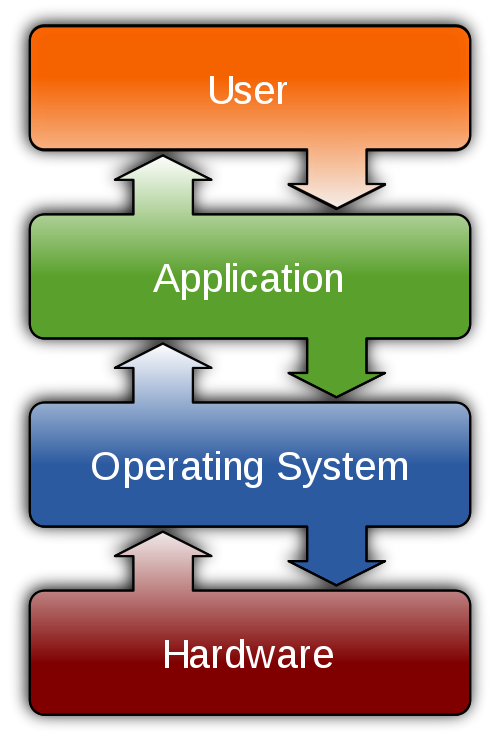
\includegraphics[height=0.5\columnwidth]{pics/OS.png}<2>%
            \end{itemize}
		\end{frame}
    \subsection{UNIX-History}
		\begin{frame}
			\frametitle{UNIX}
			\begin{itemize}
                \item<1-> Unix is a big family \\
                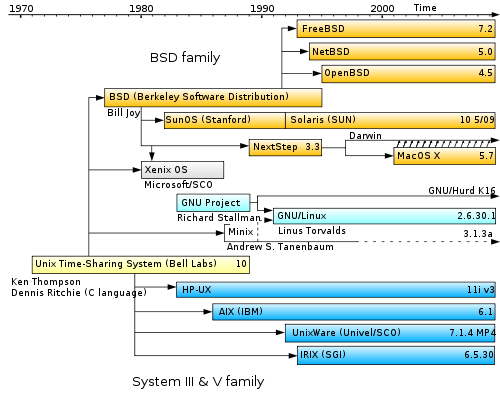
\includegraphics[height=0.6\columnwidth]{pics/500px-Unix_history.png}<2>%
            \end{itemize}
		\end{frame}
        \begin{frame}{First Linux}
            \begin{itemize}
                \item<1-> In 1991 Linux Torvalds starts writing an Terminal-Emulation for his own pleasure\\
                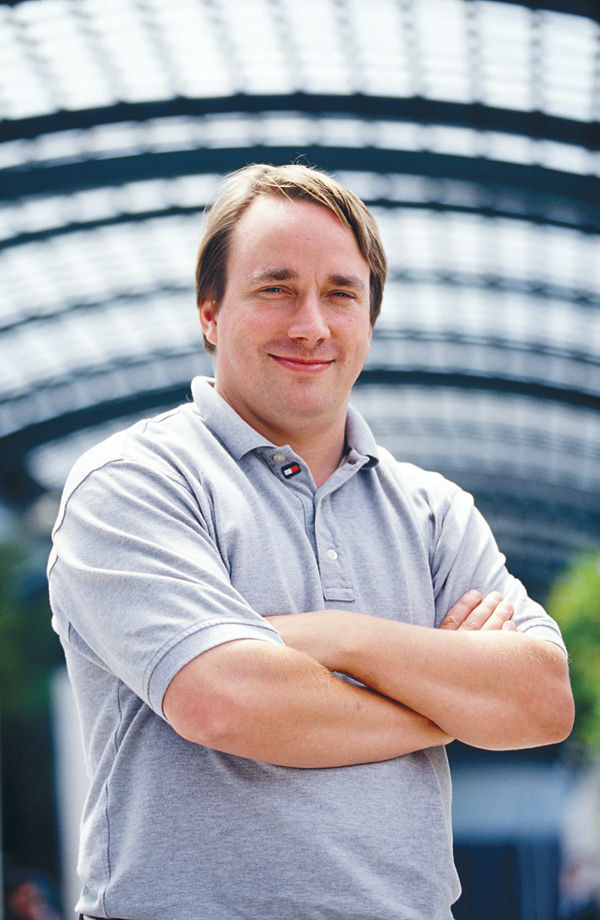
\includegraphics[height=0.3\columnwidth]{pics/Linus_Torvalds.jpg}<1->%
                \item<3-> \textbf{Fun-Fact:} Linus wants it to be called: 'Freax' or 'Buggix'. \\
                        The FTP-Admin Ari Lemmke named the folder 'Linux'
                \item<4-> First closed source, but open source when he regognize it will be cumbersome.
            \end{itemize}
        \end{frame}
    \subsection{Have a look}
        \begin{frame}{But what is UNIX?}
            \begin{itemize}
                \item<1-> A couple of components:
                \begin{itemize}
                    \item<1-> Kernel   
                    \item<2-> Development environment
                    \item<3-> Commands
                    \item<4-> Documentation
                \end{itemize}
            \end{itemize}
        \end{frame}
        \begin{frame}{Kernel}
        \begin{itemize}
            \item<1-> The main component is the Kernel
            \item<2-> it abstracts the hardware and provides basics for interaction with the computer (e.g. Process-,Memory-Management)
            \item<3-> The first free Linux-Version 0.01 (72KB) was published at October 1973 \\
                \texttt{This isn't yet the 'mother of all operating systems', and anyone who
hoped for that will have to wait for the first real release (1.0), and
even then you might not want to change from minix.}
            \item<4-> The latest Kernel-Version is 2.6.35.7 (86232KB)
        \end{itemize}
        \end{frame}
\end{document}
